\documentclass[11pt]{article}
\usepackage[a4paper,margin=1in]{geometry}
\usepackage{hyperref,enumitem,titlesec,xcolor,fancyhdr,tikz,graphicx,eso-pic}
\graphicspath{{../}}
\definecolor{kcpc-text}{RGB}{20,20,20}
\definecolor{kcpc-muted}{RGB}{90,90,90}
\definecolor{kcpc-red}{RGB}{176,0,0}
\pagestyle{fancy}\fancyhf{}
\lhead{\textcolor{kcpc-text}{\small\bfseries Papers}}
\rhead{\textcolor{kcpc-muted}{\small Week 3}}
\cfoot{\textcolor{kcpc-muted}{\small KCPC}}
\renewcommand{\headrulewidth}{0.4pt}
\renewcommand{\headrule}{\hbox to\headwidth{\color{kcpc-red}\leaders\hrule height \headrulewidth\hfill}}
\setlength{\headheight}{28pt}
\AddToShipoutPictureBG{\begin{tikzpicture}[remember picture,overlay]
  \node[opacity=0.035,at=(current page.center)]{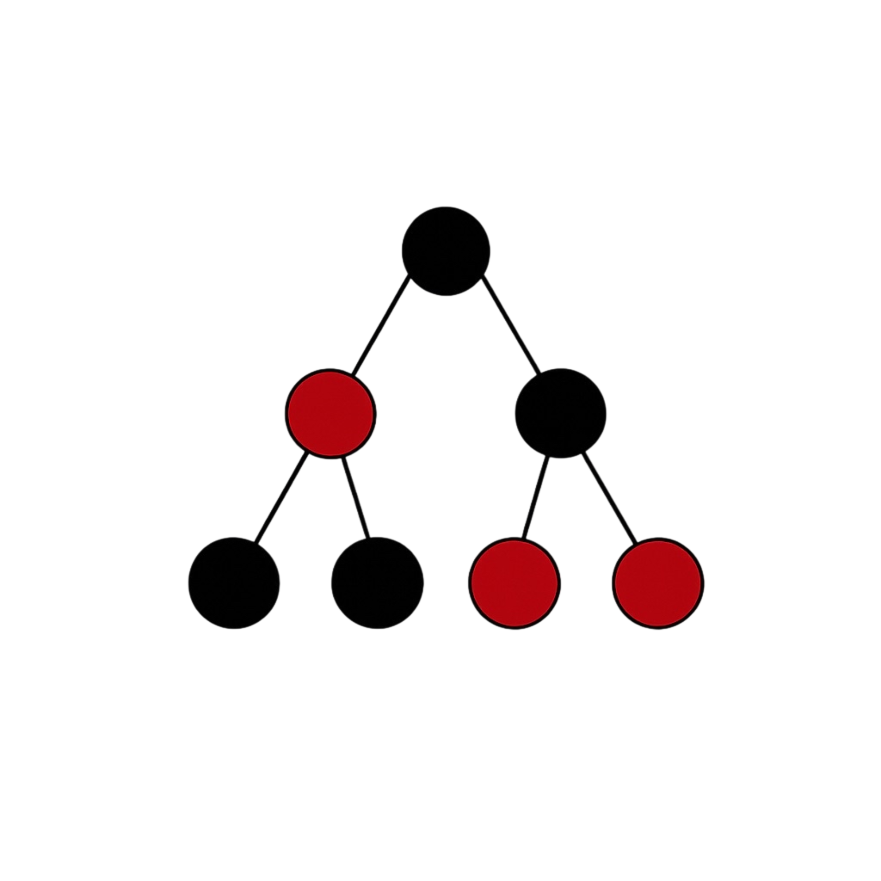
\includegraphics[width=0.38\paperwidth]{kcpc-logo.png}};
\end{tikzpicture}}
\titleformat{\section}{\large\bfseries\color{kcpc-red}}{}{0pt}{}
\title{KCPC Week 3 Papers\\Foundations of Lambda Calculus and Computation}
\author{King's Competitive Programming Club\\
  \small Curated by Mehmet Kutay Bozkurt (\href{https://github.com/mkutay}{@mkutay})}\date{}
\begin{document}
\maketitle\thispagestyle{fancy}

An annotated guide to the original research behind Workshop 3. Each entry gives a complete citation, a stable location and the part relevant to the slides and exercises. For a gentler first pass use \emph{Week 3 Reading}; the 1930s papers are primary sources, not introductory tutorials.

\section*{I. Computation and lambda-definability}
\subsection*{[1] Church, A. (1936)}
\textit{An unsolvable problem of elementary number theory.} American Journal of Mathematics, 58(2), 345--363.
\url{https://doi.org/10.2307/2371045}

\textbf{Where / why:} Pages 345--349 motivate effective calculability and lambda-definability; \S\S2--4 set up the formal apparatus. This is the historical source for treating function abstraction and application as a model of computation (slides: overview and purity). The undecidability results are beyond this workshop.

\subsection*{[2] Turing, A. M. (1936--1937)}
\textit{On computable numbers, with an application to the Entscheidungsproblem.} Proceedings of the London Mathematical Society, s2-42(1), 230--265.
\url{https://doi.org/10.1112/plms/s2-42.1.230}

\textbf{Where / why:} \S1 defines machine computation; the later discussion of computable numbers and the Entscheidungsproblem supplies the parallel machine-based notion. Read alongside Church (1936) for context for the slide's statement about describing computation, rather than as a claim that a computer literally has no numbers.

\section*{II. Reduction and substitution}
\subsection*{[3] Church, A., \& Rosser, J. B. (1936)}
\textit{Some properties of conversion.} Transactions of the American Mathematical Society, 39(3), 472--482.
\url{https://doi.org/10.2307/1989762}

\textbf{Where / why:} Pages 472--476 introduce conversion and its central consistency properties. The Church--Rosser property shows that two reduction paths can be reconciled; when a beta-normal form exists it is unique up to alpha-renaming. This underpins the slides' beta-reduction rule and the worksheet's reduction proofs.

\subsection*{[4] de Bruijn, N. G. (1972)}
\textit{Lambda calculus notation with nameless dummies, a tool for automatic formula manipulation, with application to the Church--Rosser theorem.} Indagationes Mathematicae, 34(5), 381--392 (also Proceedings, Series A, 75(5)).
\url{https://doi.org/10.1016/1385-7258(72)90034-0}

\textbf{Where / why:} Opening pages 381--383 replace bound-variable names with indices recording binder distance, removing accidental name clashes. This addresses the capture pitfall in the slides' alpha/beta formulas and Problem 3 and motivates safe substitution in interpreters.

\section*{III. Encodings and types}
\subsection*{[5] Church, A. (1940)}
\textit{A formulation of the simple theory of types.} The Journal of Symbolic Logic, 5(2), 56--68.
\url{https://doi.org/10.2307/2266170}

\textbf{Where / why:} Pages 56--58 introduce types for function application and abstraction. This contrasts the workshop's \emph{untyped} pure encodings of Boolean selectors and Church numerals with a typed formal system; useful background for later functional programming workshops.

\section*{IV. One argument at a time}
\subsection*{[6] Schönfinkel, M. (1924)}
\textit{Über die Bausteine der mathematischen Logik.} Mathematische Annalen, 92(3--4), 305--316.
\url{https://doi.org/10.1007/BF01448013}

\textbf{Where / why:} Pages 305--308 explain how multi-argument expressions can be represented by successive single-argument applications; the later pages develop combinators. This is a foundational source for the slides' currying section and selector exercises. An English translation, \emph{On the Building Blocks of Mathematical Logic}, appears in Jean van Heijenoort (ed.), \emph{From Frege to Gödel} (Harvard University Press, 1967), pp.~355--366.

For elementary definitions and reduction arguments for Boolean selectors and Church numeral arithmetic, see Selinger's \emph{Lecture Notes on the Lambda Calculus}, \S\S3.1--3.2. The supplied Ker lecture notes introduce Boolean selectors and numerals in Chapter 4, \S4.1, printed pp.~43--44; Exercises 4.1--4.2, printed p.~50, ask readers to construct AND and verify a predecessor, including its zero case. See \emph{Week 3 Reading} for the links. These lecture notes are secondary expositions, so they are listed in the reading guide rather than treated as original research papers.

\end{document}
